% =============================================================================
%
% This is the LaTeX source code of the lecture notes.
%
%
% Author:   Blazej Bucha
% Year:     2022
% Contact:  blazej.bucha@stuba.sk
% Encoding: UTF-8
%
% =============================================================================






% LaTeX Packages
% =============================================================================

\documentclass[a4paper, 12pt]{book}
\usepackage[slovak]{babel}
\usepackage[utf8]{inputenc}
\usepackage[round]{natbib}
\usepackage{amsmath}
\usepackage{upgreek}
\usepackage{listings}
\usepackage{xcolor}
\usepackage{graphicx}
\usepackage{accsupp}
\usepackage[top=2.5cm, bottom=2.5cm, left=2.5cm, right=2.5cm]{geometry}
\linespread{1.2}

% =============================================================================






% Define and set the style of code listings
% =============================================================================

% Define custom colours
\definecolor{comments}{rgb}{0.65, 0.65, 0.65}
\definecolor{strings}{rgb}{0.0, 0.3, 0.7}
\definecolor{linenumbers}{rgb}{0.5, 0.5, 0.5}
\definecolor{keywords}{rgb}{0.85, 0.0, 0.0}
\definecolor{backcolour}{rgb}{0.98, 0.98, 0.98}


% Define custom listing style
\lstdefinestyle{codestyle}
{
    backgroundcolor=\color{backcolour},
    commentstyle=\color{comments},
    keywordstyle=\color{keywords},
    numberstyle=\tiny\noncopynumber,
    columns=flexible,
    stringstyle=\color{strings},
    basicstyle=\ttfamily\footnotesize,
    breakatwhitespace=false,
    breaklines=true,
    captionpos=b,
    keepspaces=true,
    numbers=left,
    numbersep=5pt,
    showspaces=false,
    showstringspaces=false,
    showtabs=false,
    tabsize=2
}


% Defines a new command that ensures we can copy the source code from the 
% compiled PDF without copying the line numbers
\newcommand{\noncopynumber}[1]
{
    \BeginAccSupp{method=escape,ActualText={}}
    #1
    \EndAccSupp{}
}


% Apply the custom listing style
\lstset{style=codestyle}


% It seems the "listings" package is not able to encode the nice special Slovak 
% characters such as "á", "ľ", etc.  Next follows a brute force solution.
\lstset{
  literate={á}{{\'a}}1
           {ä}{{\" a}}1
           {č}{{\v c}}1
           {ď}{{d\kern-0.07cm\char39\kern-0.07cm}}1
           {é}{{\'e}}1
           {í}{{\'i}}1
           {ĺ}{{\'l}}1
           {ľ}{{l\kern-0.12cm\char39\kern-0.05cm}}1
           {ň}{{\v n}}1
           {ó}{{\'o}}1
           {ô}{{\^o}}1
           {ŕ}{{\'r}}1
           {š}{{\v s}}1
           {ť}{{t\kern-0.10cm\char39\kern-0.05cm}}1
           {ú}{{\'u}}1
           {ý}{{\'y}}1
           {ž}{{\v z}}1
           {Á}{{\'A}}1
           {Ä}{{\" A}}1
           {Č}{{\v C}}1
           {Ď}{{\v D}}1
           {É}{{\'E}}1
           {Í}{{\'I}}1
           {Ĺ}{{\'L}}1
           {Ľ}{{L\kern-0.12cm\char39\kern-0.00cm}}1
           {Ň}{{\v N}}1
           {Ó}{{\'O}}1
           {Ô}{{\^O}}1
           {Ŕ}{{\'R}}1
           {Š}{{\v S}}1
           {Ť}{{\v T}}1
           {Ú}{{\'U}}1
           {Ý}{{\'Y}}1
           {Ž}{{\v Z}}1
}


% Add the "as" keyword to the Python listings
\lstdefinelanguage{mypython}[]{Python}{morekeywords={as,True,False}}


% Caption title for listings
\renewcommand\lstlistingname{Zdrojový kód}

% =============================================================================






% Custom commands
% =============================================================================
\newcommand{\diff}{\mathrm d}
\newcommand{\grad}{\mathrm{grad}}
\newcommand{\gidx}{\mathrm g}
\let\vec\mathbf
% =============================================================================






% =============================================================================

\sloppy
\begin{document}

% -----------------------------------------------------------------------------
\tableofcontents
\newpage
% -----------------------------------------------------------------------------






% -----------------------------------------------------------------------------

\chapter*{Úvod}






% -----------------------------------------------------------------------------

\chapter{Fyzikálna geodézia}

Tvar Zeme možno definovať niekoľkými spôsobmi v závislosti od kontextu 
\citep{MoritzTheFigureOfTheEarth}.  Azda najprirodzenejšie je definovať tvar 
Zeme jej skutočným fyzickým povrchom, teda tou časťou Zeme, ktorá je viditeľná 
voľným okom.  Takýto povrch by však obsahoval aj nespočetné množstvo zložitých 
terénnych útvarov, napríklad náhle skokovité zmeny terénu.  Hoci sú takéto 
oblasti krásne na pohľad, znemožňujú aplikovať časť potrebného matematického 
aparátu, napríklad plošnú integráciu.  Skúmať takto chápaný zemský povrch je 
preto možné až po istom vyhladení.  Napriek tomu, ide o veľmi komplexnú plochu.

Pri definovaní tvaru Zeme však môžeme vziať v úvahu skutočnosť, že približne 
dve tretiny zemského povrchu tvorí voda v podobe oceánov a morí.  Ak by sme 
s podobnou mierou hladkosti dokázali predĺžiť povrch oceánov a morí aj popod, 
resp. ponad pevnú časť zemského povrchu, získali by sme v porovnaní s fyzickým 
povrchom Zeme značne jednoduchší a hladší, no pritom stále verný tvar Zeme.  
Voda má za istých okolností navyše tú výhodnú vlastnosť, že existuje fyzikálna 
veličina, ktorá je na jej povrchu konštantná.  Táto vlastnosť by teda následne 
mohla umožniť akúsi predikciu morskej hladiny aj popod, resp. ponad kontinenty.  
Inými slovami, v tejto definícií tvaru Zeme by išlo o geometricky jednoduchšiu 
plochu, navyše tentokrát už aj s istými relatívne jednoducho popísateľnými 
fyzikálnymi vlastnosťami.  Takto definovaný tvar Zeme bol navrhnutý 
C. F. Gaussom (1777--1855) a podľa návrhu J. B. Listinga (1808--1882) ho 
nazývame \emph{geoid}.  Veličina, ktorá je konštantná na povrchu geoidu sa 
nazýva \emph{tiažový potenciál}.

\emph{Fyzikálna geodézia} je vedná disciplína zaoberajúca sa určovaním tvaru 
Zeme, jej tiažovým poľom a ich zmenami v čase.  Študované sú oba vyššie opísané 
prístupy k tvaru Zeme, pričom historicky bol predmetom záujmu ako prvý geoid.  
Hoci prirodzená, no matematicky odvážna myšlienka určovať priamo fyzický povrch 
Zeme pochádza už od E. H. Brunsa (1848--1919), do popredia záujmu ju dostal až 
v polovici 20. storočia M. S. Molodenskij (1909--1991).  Dôležitá je však 
skutočnosť, že i v tomto prípade je tvar Zeme určovaný z informácie o tiažovom 
poli.  Študovať tvar Zeme, čo je jedna zo základných úloh geodézie, teda 
znamená študovať aj tiažové pole Zeme.

\section{Newtonov integrál}

%Uvažujme hmotný bod o hmotnosti $m$.  V zmysle gravitačného zákona 
%formulovaného I. Newtonom (1642--1727) tento hmotný bod generuje gravitačný 
%potenciál $V$.  Vo vzdialenosti $l$ od tohto hmotného je gravitačný potenciál 
%daný vzťahom
%%
%\begin{equation}
%V = G \frac{m}{l}{,}
%\end{equation}
%%
%kde $G = 6.6742 \times 10^{-11} \ \mathrm{m}^3 \ \mathrm{kg}^{-1} 
%\ \mathrm{s}^{-2}$ je Newtonova gravitačná konštanta.

Dva hmotné body $P$ a $Q$ nachádzajúce sa od seba vo vzdialenosti $l$ sa 
navzájom priťahujú \emph{gravitačnou silou}
%
\begin{equation}
\label{eq:gravitational_law}
\vec F = -G \frac{m_P \, m_Q}{l^2} \, \frac{\vec r}{l}{.}
\end{equation}
%
Symbol $G$ označuje gravitačnú konštantu, $m_P$ a $m_Q$ predstavujú hmotnosti 
hmotných bodov a $\vec r$ je vektor definovaný bodmi $P$ a $Q$ so začiatkom 
v~bode $Q$.  Záporné znamienko v rovnici znamená, že vektor sily $\vec F$ má 
začiatok v bode $P$ a smeruje do bodu $Q$.

Rovnica~(\ref{eq:gravitational_law}) predstavuje \emph{gravitačný zákon} formulovaný 
I. Newtonom (1642--1727).  Hovorí, že dva ľubovoľné hmotné body sú vzájomne 
priťahované silou, ktorej veľkosť je priamo úmerná súčinu ich hmotností 
a nepriamo úmerná štvorcu ich vzájomnej vzdialenosti.  \emph{Hmotný bod} je 
idealizovaný pojem predstavujúci časticu s nulovým rozmerom a konečnou 
nenulovou hmotnosťou bez akýchkoľvek ďalších vlastností či štruktúry.  
Rovnicu~(\ref{eq:gravitational_law}) možno s rozumnou mierou aproximácie aplikovať 
napr. na popis pohybu planét Slnečnej sústavy.  Rozmery týchto telies sú totiž 
natoľko zanedbateľné v porovnaní s ich vzájomnou vzdialenosťou, že sa 
nedopustíme nerozumne veľkej chyby, ak hmotnosti týchto telies sústredíme do 
ich ťažiska a úplne zanedbáme ich tvar.  Gravitačnú silu je možné skúmať aj 
s použitím bežnejších hmotností a vzdialeností.  Hodnota gravitačnej konštanty
%
\begin{equation}
G = (6.67430 \pm 0.00015) \times 10^{-11} \ \mathrm{m}^3 \ \mathrm{kg}^{-1} 
\ \mathrm{s}^{-2}
\end{equation}
%
spolu s rovnicou~(\ref{eq:gravitational_law}) však veľmi rýchlo napovedia, že 
gravitačná sila bude v takom prípade veľmi malá, v mnohých geodetických 
aplikáciach dokonca zanedbateľná.  Napriek tomu, súčasnými geodetickými 
prístrojmi je predsa len možné zaznamenať gravitačný vplyv dokonca i tak malých 
objektov, akými sú budova, auto, či dospelý človek.  Čím má objekt menšiu 
hmotnosť, tým bližšie (pozri rovnicu~\ref{eq:gravitational_law}) sa musí nachádzať 
pri meracom zariadení, aby bol jeho vplyv merateľný geodetickými prístrojmi.  
V prípade dospelého človeka ide o vzdialenosti niekoľkých desiatok, či stoviek 
centimetrov.

Newtonov gravitačný zákon je ale v zhode so špecializovanými presnými meraniami 
i v prípade tak malých vzdialeností ako $52\ \upmu\mathrm{m}$ \citep{Lee2020}.  
Táto skutočnosť je pozoruhodná, obzvlášť ak uvážime, že tento zákon bol 
odpozorovaný z pohybu nebeských telies po oblohe.  Popisuje Newtonov gravitačný 
zákon dostatočne presne realitu ešte aj na menšej subatomárnej úrovni?  Všetko 
nasvedčuje tomu, že nie.  Nie je to však prekvapivé, keďže \emph{Newtonov 
gravitačný zákon je nesprávny}.  Podľa Newtonovej teórie je napríklad 
gravitačný vplyv okamžitý, čo je v rozpore s experimentálne potvrdenou 
Einsteinovou teóriou relativity.  Tá hovorí, že žiadny signál, a teda ani ten 
gravitačný, nie je možné poslať rýchlosťou väčšou ako je rýchlosť svetla.  
Neplatnosť Newtonovej teórie gravitácie bola dokázaná nezávislými experimentmi.  
Pre účely fyzikálnej geodézie sú však aproximácie v Newtonovom gravitačnom 
zákone zanedbateľné, pretože sú nemerateľné bežnými geodetickými prístrojmi.  
Navyše, táto teória ešte stále veľmi dobre a jednoducho popisuje obrovské 
množstvo experimentálnych meraní, medzi inými aj tých geodetických.  Azda nič 
by preto nemalo brániť pôžitku zo skúmania tohto viac ako tristoročného zákona 
opisujúceho gravitáciu.

\subsection{Gravitačné zrýchlenie}

Rovnica~(\ref{eq:gravitational_law}) závisí od hmotnosti oboch hmotných bodov.  
Predpokladajme však, že predmetom nášho záujmu je iba gravitačné pole 
generované hmotným bodom~$Q$.  Skúmať takéto pole je možné po normovaní vektora 
gravitačnej sily hmotnosťou hmotného bodu $P$,
%
\begin{equation}
\frac{\vec F}{m_P}{,}
\end{equation}
%
prípadne aplikáciou podmienky $m_P = 1\ \mathrm{kg}$.  Oba spôsoby vedú 
ekvivalentne k veličine, ktorá sa nazýva \emph{gravitačné zrýchlenie},
%
\begin{equation}
\label{eq:gravitational_vector}
\vec g_\gidx(P) = -G \frac{m}{l^2} \, \frac{\vec r}{l}{,}
\end{equation}
%
pričom $m = m_Q$.  Vektor gravitačného zrýchlenia teda nezávisí od hmotnosti 
hmotného bodu, v ktorom skúmame gravitačné pole, má začiatok v bode $P$ 
a smeruje do bodu $Q$.  V súvislosti s hmotným bodom $P$ je preto možné pre 
jednoduchosť vynechať prívlastok \emph{hmotný} a považovať $P$ za geometrický 
bod bez fyzikálnych vlastností.

Ak by sme chceli v bode $P$ vypočítať gravitačné zrýchlenie generované $N$ 
hmotnými bodmi, vektorovo sčítame jednotlivé vektory gravitačného zrýchlenia, 
teda
%
\begin{equation}
\label{eq:gravitational_vector_N_point_masses}
\vec g_\gidx(P) = \sum_{i = 0}^{N}\vec g_{\gidx,i}(P) = -G \sum_{i = 0}^{N} 
\frac{m_i}{l_i^2} \, \frac{\vec r_i}{l_i}{.}
\end{equation}

Newtonov gravitačný zákon formulovaný tak, ako v predchádzajúcej kapitole platí 
spolu s rovnicami~(\ref{eq:gravitational_vector}) 
a (\ref{eq:gravitational_vector_N_point_masses}) iba pre hmotné body.  
K vernejšiemu popisu reality sa dostaneme, keď opustíme koncept hmotných bodov 
a začneme skúmať gravitačne pole generované telesom, ktoré má konečný objem 
$\tau$ a ohraničenú hustotu $\rho$.  Takéto teleso budeme nazývať 
\emph{všeobecné teleso}.  Gravitačné zrýchlenie všeobecného telesa je dané 
vzťahom
%
\begin{equation}
\label{eq:gravitational_vector_integral}
\vec g_\gidx(P) = -G \iiint_{\tau} \frac{\vec r}{l^3} \, \rho \, \diff\tau{,}
\end{equation}
%
pričom bol použitý vzťah $\diff m = \rho \, \diff \tau$.  Symbol $\vec r$ 
tentokrát predstavuje vektor daný výpočtovým bodom $P$ a diferenciálnym objemom 
$\diff\tau$ so začiatkom v $\diff\tau$ a $l = | \vec r |$ je opäť jeho veľkosť.  
Dôležité je spomenúť, že hustota $\rho$ môže byt funkciou polohy 
diferenciálneho elementu $\diff\tau$.

Vektor gravitačného zrýchlenia veľmi úzko súvisí s veličinou, ktorú je možné 
odmerať na povrchu Zeme, a tak má pre fyzikálnu geodéziu kľúčový význam.

\subsection{Gravitačný potenciál}

Gravitačné zrýchlenie $\vec g_\gidx$ je vektorová veličina.  Skalárna veličina 
gravitačného poľa sa nazýva \emph{gravitačný potenciál} a označuje sa symbolom 
$V$.  Pre porozumenie vzťahu medzi týmito dvoma veličinami je potrebné 
predstaviť diferenciálny operátor gradient.

\subsubsection{Operátor gradient}

\emph{Gradient} je diferenciálny operátor, ktorý je v trojrozmernom pravouhlom 
súradnicovom systéme $(x, y, z)$ definovaný nasledovne,
%
\begin{equation}
\label{eq:gradient}
\nabla = \grad = \vec e_1 \frac{\partial}{\partial x} + \vec e_2 
\frac{\partial}{\partial y} + \vec e_3 \frac{\partial}{\partial z} =
\begin{bmatrix}
\dfrac{\partial}{\partial x} \\[2ex]
\dfrac{\partial}{\partial y} \\[2ex]
\dfrac{\partial}{\partial z}
\end{bmatrix}
{,}
\end{equation}
%
kde $\vec e_1$, $\vec e_2$ a $\vec e_3$ sú jednotkové vektory rovnobežné so 
smerom súradnicových osí $x$, $y$ a $z$.  Aplikáciou operátora gradient na 
skalárnu funkciu $f$ teda získame vektorovú funkciu
%
\begin{equation}
\vec f(x, y, z) = \nabla f(x, y, z) = \grad \ f(x, y, z) = \begin{bmatrix}
\dfrac{\partial f(x, y, z)}{\partial x} \\[2ex]
\dfrac{\partial f(x, y, z)}{\partial y} \\[2ex]
\dfrac{\partial f(x, y, z)}{\partial z}
\end{bmatrix}
{,}
\end{equation}
%
ktorá udáva smer a veľkosť najväčšieho nárastu funkcie $f$ v bode so 
súradnicami $x$, $y$ a $z$.

Uvažujme dvojrozmerný pravouhlý súradnicový systém, v ktorom je definovaná 
skalárna funkcia
%
\begin{equation}
\label{eq:f}
f(x, y) = \sin(2x) + \cos(2y){.}
\end{equation}
%
Aplikáciou operátora gradient získame v zmysle rovnice~(\ref{eq:gradient}) 
vektorovú funkciu
%
\begin{equation}
\label{eq:gradf}
\vec f(x, y) =
\begin{bmatrix}
\dfrac{\partial f(x, y)}{\partial x} \\[2ex]
\dfrac{\partial f(x, y)}{\partial y}
\end{bmatrix}
=
\begin{bmatrix}
2 \cos(2x) \\[2ex]
-2 \sin(2y)
\end{bmatrix}
{.}
\end{equation}
%
Ukážka numerického výpočtu funkcie~(\ref{eq:f}) a jej 
gradientu~(\ref{eq:gradf}) na~intervale $x, y \in [-1, 1]$ je uvedená 
v Zdrojovom~kóde~\ref{src:f_gradf}.  Grafické znázornenie je uvedené na 
Obr.~\ref{fig:f_gradf}.

\lstinputlisting[caption=Výpočet a~zobrazenie funkcie dvoch premenných a~jej 
gradientu v programovacom jazyku Python, language=mypython, label=src:f_gradf, 
captionpos=t]{../python/f-gradf.py}

\begin{figure}[bt]
\centering
\includegraphics{../figs/f-gradf.pdf}
\caption{Skalárna funkcia $f(x, y) = \sin(2x) + \cos(2y)$ a~jej gradient 
$\nabla f(x, y)$ na~intervale $x, y \in [-1, 1]$.  Skalárna funkcia je 
znázornená hypsometricky.  Gradient je zobrazený orientovanými šípkami, pričom 
smer šípky udáva smer najväčšieho nárastu funkcie $f(x, y)$ v danom bode 
a dĺžka šípky znázorňuje veľkosť nárastu ***FAREBNA SKALA***}
\label{fig:f_gradf}
\end{figure}


%
\begin{equation}
\label{eq:newton}
V(P) = G \iiint_{\tau} \frac{\rho(Q)}{l(P, Q)} \diff \tau(Q){,}
\end{equation}
%
následne hľadať veličiny, ktoré sú s ním spojené a je možné ich odmerať, 
a nakoniec zo získaných meraní vypočítať tvar Zeme v zmysle zvolenej definície.

\begin{figure}[bt]
\centering
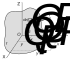
\includegraphics{../figs/gravitating-body/gravitating-body.pdf}
\caption{Všeobecné teleso a výpočtový bod $P$ ***VEKTOR R***}
\end{figure}

Vo vzťahu (\ref{eq:newton}) predstavuje symbol $V$ gravitačný potenciál v bode 
$P$ generovaný telesom s objemom $\tau$ a hustotou $\rho(P')$, ktorá môže 
závisieť od polohy integračného elementu $\diff \tau(P')$ vo vnútri telesa.  
Symbolom $l$ budeme označovať Euklidovskú vzdialenosť, v tomto prípade medzi 
výpočtovým bodom $P$ a integračným elementom $\diff \tau(P')$ vo vnútri telesa, 
ktoré generuje gravitačne pole.







\section{Súradnicový systém}

\begin{figure}[bt]
\centering
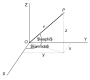
\includegraphics{../figs/coordinate-systems/cart-sph.pdf}
\caption{Pravouhlé a~sférické súradnice}
\end{figure}


\section{Polia}

\section{Operátory poľa}

% čo to je?
% súradnicový systém?
% polia
% skalár, vektor, tenzor + ukážky + kódy
% gradient, divergencia, rotácia
% Newtonov gravitačný zákon + pár slov k teórii relativity






% -----------------------------------------------------------------------------

\chapter{Gravitačné a tiažové pole homogénnej gule}

% polia, označenia, jednotky





% -----------------------------------------------------------------------------

\chapter{Gravitačný potenciál všeobecného telesa}

% rozvoj potenciálu do radu sférických harmonických funkcií






% -----------------------------------------------------------------------------

\chapter{Sférické harmonické funkcie}

% čo to je, definícia, porovnanie s jednotkovými vektormi, delenie, ukážka 
% sférických harmonických funkcií v matematickom zápise + obrázky + kód, 
% normovanie, Legendreove polynómy + funkcie, definícia, grafy + kód

\lstinputlisting[caption=Výpočet a~zobrazenie Legendreových polynómov, 
language=mypython]{../python/legendre-polynomials.py}

\begin{figure}[bt]
\centering
\includegraphics{../figs/legendre-polynomials.pdf}
\caption{Legendreove polynómy}
\end{figure}


\lstinputlisting[caption=Výpočet a~zobrazenie nenormovaných sférických 
harmonických funkcií, language=mypython]{../python/spherical-harmonics.py}

\begin{figure}[bt]
\centering
\includegraphics{../figs/spherical-harmonic-n3-m0.pdf}
\includegraphics{../figs/spherical-harmonic-n3-m1.pdf}
\includegraphics{../figs/spherical-harmonic-n3-m3.pdf}
\includegraphics{../figs/spherical-harmonic-n4-m0.pdf}
\includegraphics{../figs/spherical-harmonic-n4-m1.pdf}
\includegraphics{../figs/spherical-harmonic-n4-m4.pdf}
\caption{Nenormované plošné sférické harmonické funkcie.  Záporné hodnoty sú 
zobrazené odtieňmi modrej farby, kladné hodnoty odtieňmi červenej farby.  
\textit{Vrchný rad} (zľava): $Y_{3,0}(\varphi, \lambda)$, $Y_{3,1}(\varphi, 
\lambda)$, $Y_{3,3}(\varphi, \lambda)$.  \textit{Spodný rad} (zľava): 
$Y_{4,0}(\varphi, \lambda)$, $Y_{4,1}(\varphi, \lambda)$, $Y_{4,4}(\varphi, 
\lambda)$}
\label{fig:sh}
\end{figure}


\begin{figure}[bt]
\centering
\includegraphics{../figs/spherical-harmonic-n3-m0-3d.pdf}
\includegraphics{../figs/spherical-harmonic-n3-m1-3d.pdf}
\includegraphics{../figs/spherical-harmonic-n3-m3-3d.pdf}
\includegraphics{../figs/spherical-harmonic-n4-m0-3d.pdf}
\includegraphics{../figs/spherical-harmonic-n4-m1-3d.pdf}
\includegraphics{../figs/spherical-harmonic-n4-m4-3d.pdf}
\caption{Nenormované plošné sférické harmonické funkcie z Obr.~\ref{fig:sh} 
zobrazené ako odľahlosť nadobúdanej hodnoty od jednotkovej sféry}
\label{fig:sh3d}
\end{figure}





% -----------------------------------------------------------------------------

\section{Elipsoidické harmonické funkcie}

% čo to je, definícia, obrázky + grafy + kód, využitie






% -----------------------------------------------------------------------------

\chapter{Normálne tiažové pole}

% čo to je, prečo sa zavádza, ekvipotenciálny elipsoid, základné a odvodené 
% parametre elipsoidu, geometrické a fyzikálne parametre, základné veličiny, 
% stručne opísať normálne pole pomocou elipsoidických harmonických funkcií 
% a vysvetliť výhody takéhoto opisu (uzavreté vzťahy), somiglianov vzťah






% -----------------------------------------------------------------------------

\chapter{Poruchové pole}

% čo to je, prečo sa zavádza, využitie, základné veličiny, vzťahy medzi nimi






% -----------------------------------------------------------------------------

\chapter{Výpočet geoidu}






% -----------------------------------------------------------------------------

\section{Výpočet geoidu rozvojom do radu sférických harmonických funkcií}






% -----------------------------------------------------------------------------

\section{Výpočet geoidu astronomicko--geodetickou niveláciou}






% -----------------------------------------------------------------------------

\section{Výpočet geoidu numerickou integráciou Stokesovho a Hotine integrálov}






% -----------------------------------------------------------------------------

\chapter*{Záver}






% Bibliography
% -----------------------------------------------------------------------------

\bibliographystyle{apalike}
\bibliography{references.bib}

\end{document}

% =============================================================================
% End of the code

